% Created 2018-03-10 sáb 19:19
% Intended LaTeX compiler: pdflatex
\documentclass[xcolor={usenames,svgnames,dvipsnames}]{beamer}
\usepackage[utf8]{inputenc}
\usepackage[T1]{fontenc}
\usepackage{graphicx}
\usepackage{grffile}
\usepackage{longtable}
\usepackage{wrapfig}
\usepackage{rotating}
\usepackage[normalem]{ulem}
\usepackage{amsmath}
\usepackage{textcomp}
\usepackage{amssymb}
\usepackage{capt-of}
\usepackage{hyperref}
\usepackage{color}
\usepackage{listings}
\usepackage{mathpazo}
\usepackage{gensymb}
\usepackage{amsmath}
\usepackage{chemarr}%flechas para reacciones químicas (SFER.tex)
\bibliographystyle{plain}
\AtBeginSubsection[]{\begin{frame}[plain]\tableofcontents[currentsubsection,sectionstyle=show/shaded,subsectionstyle=show/shaded/hide]\end{frame}}
\AtBeginSection[]{\begin{frame}[plain]\tableofcontents[currentsection,hideallsubsections]\end{frame}}
\usepackage[emulate=units]{siunitx}
\sisetup{fraction=nice, decimalsymbol=comma, retain-unity-mantissa = false}
\newunit{\wattpeak}{Wp}
\newunit{\watthour}{Wh}
\newunit{\amperehour}{Ah}
\hypersetup{colorlinks=true, linkcolor=Blue, urlcolor=Blue}
\renewcommand{\thefootnote}{\fnsymbol{footnote}}
\setbeamercolor{alerted text}{fg=blue!50!black} \setbeamerfont{alerted text}{series=\bfseries}
\usetheme[hideothersubsections]{Goettingen}
\usecolortheme{rose}
\usefonttheme{serif}
\author{Oscar Perpiñán Lamigueiro \\ \url{http://oscarperpinan.github.io}}
\date{}
\title{Célula Solar}
\subtitle{Energía Solar Fotovoltaica}
\hypersetup{
 pdfauthor={Oscar Perpiñán Lamigueiro \\ \url{http://oscarperpinan.github.io}},
 pdftitle={Célula Solar},
 pdfkeywords={},
 pdfsubject={},
 pdfcreator={Emacs 25.2.2 (Org mode 9.1.6)}, 
 pdflang={Spanish}}
\begin{document}

\maketitle

\section{Teoría de Semiconductores}
\label{sec:org17e37aa}
\subsection{Conducción eléctrica}
\label{sec:org26e5b74}

\begin{frame}[label={sec:orgc16b482}]{Bandas de energía}
\begin{itemize}[<+->]
\item En un \alert{sólido} el número de átomos es tan elevado que los niveles de energía forman \alert{bandas continuas de energía}.

\item Los \alert{electrones} asociados a los átomos del sólido \alert{llenan estas bandas en orden ascendente}.

\item La banda de mayor energía completamente ocupada se denomina \alert{banda de valencia} (\emph{electrones ligados a átomos}).

\item La siguiente banda, parcialmente ocupada o vacía, se denominada \alert{banda de conducción} (\emph{electrones desligados de átomos}).

\item Estas bandas pueden estar separadas por otra banda de energías que corresponde a \alert{estados no permitidos} (\alert{banda prohibida}), o \alert{pueden estar solapadas} permitiendo una transición fácil de una a otra.
\end{itemize}
\end{frame}

\begin{frame}[label={sec:org58f037e}]{Bandas de energía}
\begin{center}


\begin{center}
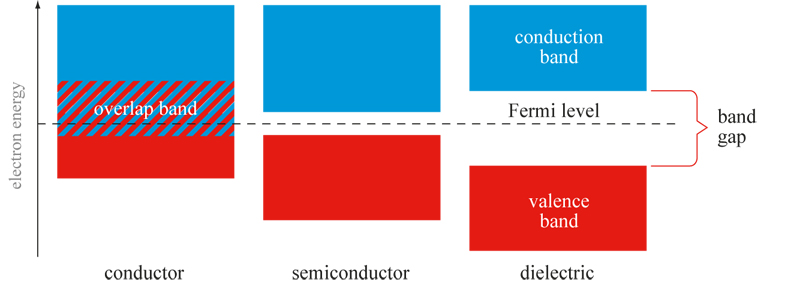
\includegraphics[width=.9\linewidth]{../figs/simplified_band_diagram.jpg}
\end{center}
\end{center}
\footnotetext[2]{http://commons.wikimedia.org/}
\end{frame}

\begin{frame}[label={sec:org575492f}]{Conductores, aislantes y semiconductores}
Las \alert{propiedades eléctricas} del sólido dependen de esta \alert{posición relativa entre bandas}.
\begin{itemize}[<+->]
\item En un \alert{conductor} la \(E_{g}\) es muy baja y los electrones circulan fácilmente por la banda de conducción.

\item En un \alert{aislante} se necesita una cantidad de energía muy alta para que los electrones puedan acceder a la banda de conducción   (\(E_{g}>\SI{5}{\electronvolt}\))

\item En un \alert{semiconductor} la \(E_{g}\) es baja (\(E_{g}<\SI{5}{\electronvolt}\)): los electrones pueden \guillemotleft{}saltar\guillemotright{} a la banda de conducción con un aporte energético.

\begin{itemize}
\item \(E_{g}(Si)=\SI{1.12}{\electronvolt}\)

\item \(E_{g}(AsGa)=\SI{1.4}{\electronvolt}\)
\end{itemize}
\end{itemize}
\end{frame}

\begin{frame}[label={sec:orgf5c5a68}]{Conductores, aislantes y semiconductores}
\begin{block}{La conductividad de los materiales depende de la \alert{concentración de electrones libres} (n) presentes en la banda de conducción}
\end{block}

\begin{block}{Valores típicos de n}
\begin{itemize}
\item Metal: \SI{1e22}{\per\cm\cubed}
\item Aislante: \SI{10}{\per\cm\cubed}
\item Semiconductor: \SI{1e10}{\per\cm\cubed} a T = \SI{300}{\kelvin}
\end{itemize}
\end{block}
\end{frame}

\subsection{Semiconductores}
\label{sec:org5ef309c}

\begin{frame}[label={sec:org8891d3c}]{Red cristalina de Si (T = \SI{0}{\kelvin})}
\begin{center}
\begin{center}
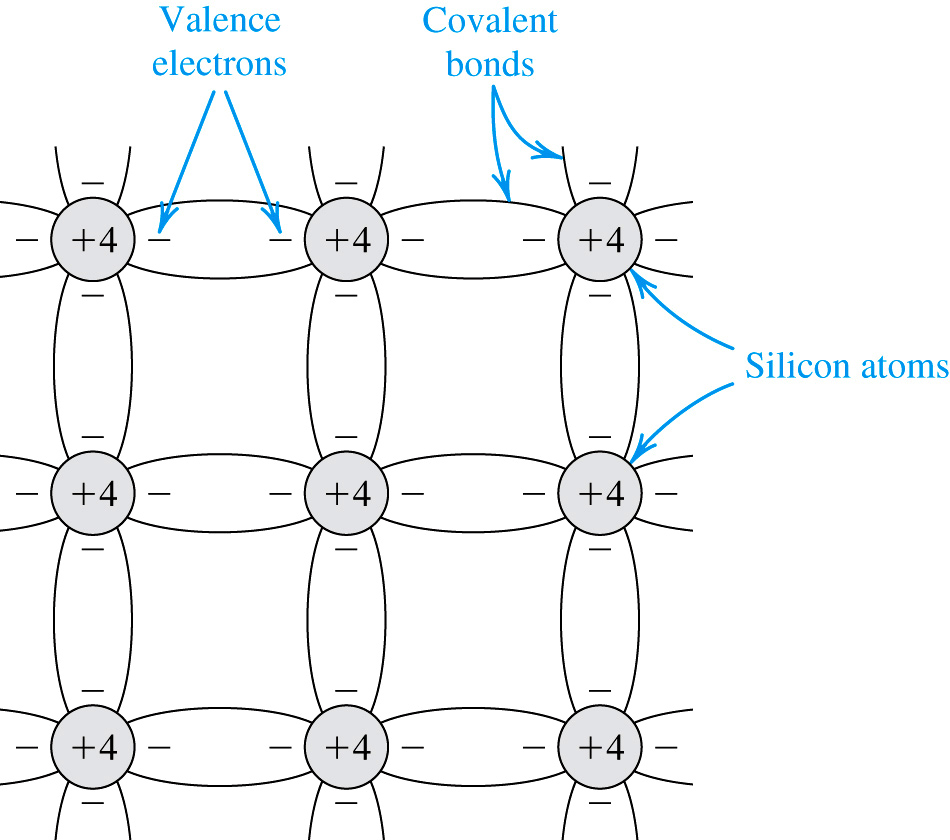
\includegraphics[width=.9\linewidth]{../figs/silicio_T0K.jpg}
\end{center}
\end{center}
\footnotetext[2]{Figura de Sedra and Smith, Microelectronic Circuits}
\end{frame}
\begin{frame}[label={sec:org6816c73}]{Generación de electrón-hueco (T > \SI{0}{\kelvin})}
\begin{center}
\begin{center}
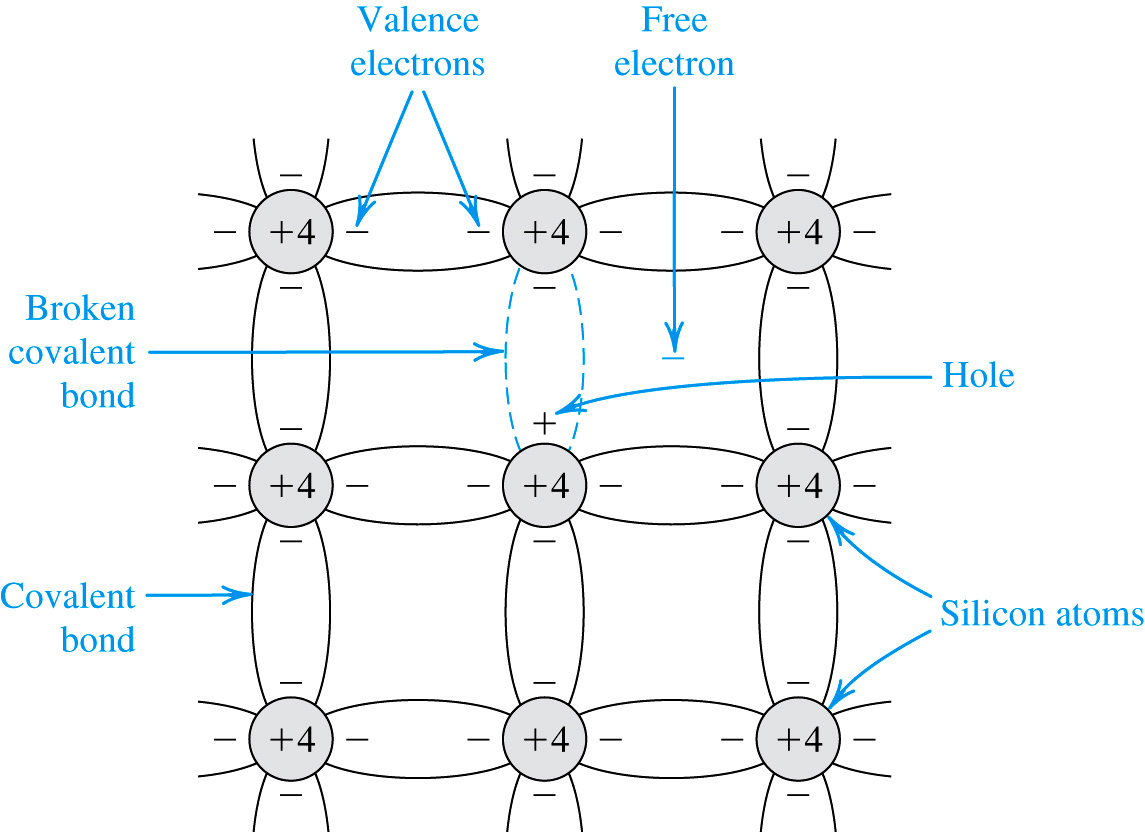
\includegraphics[width=.9\linewidth]{../figs/silicio_T300K.jpg}
\end{center}
\end{center}
\footnotetext[2]{Figura de Sedra and Smith, Microelectronic Circuits}
\end{frame}
\begin{frame}[plain,label={sec:orgd669f9a}]{Generación de electrón-hueco}
\begin{columns}
\begin{column}{0.7\columnwidth}
\begin{itemize}[<+->]
\item Cuando se \alert{rompe un enlace}, un electrón y un hueco quedan libres para moverse por el material (conducción intrínseca).

\item Esta \alert{circulación es aleatoria}, sin una dirección predeterminada: \alert{no es aprovechable} en un circuito externo.

\item La \alert{densidad intrínseca de huecos y electrones es idéntica} (depende de la temperatura y de \(E_{g}\)).
\end{itemize}
\end{column}
\begin{column}{0.6\columnwidth}
\begin{center}
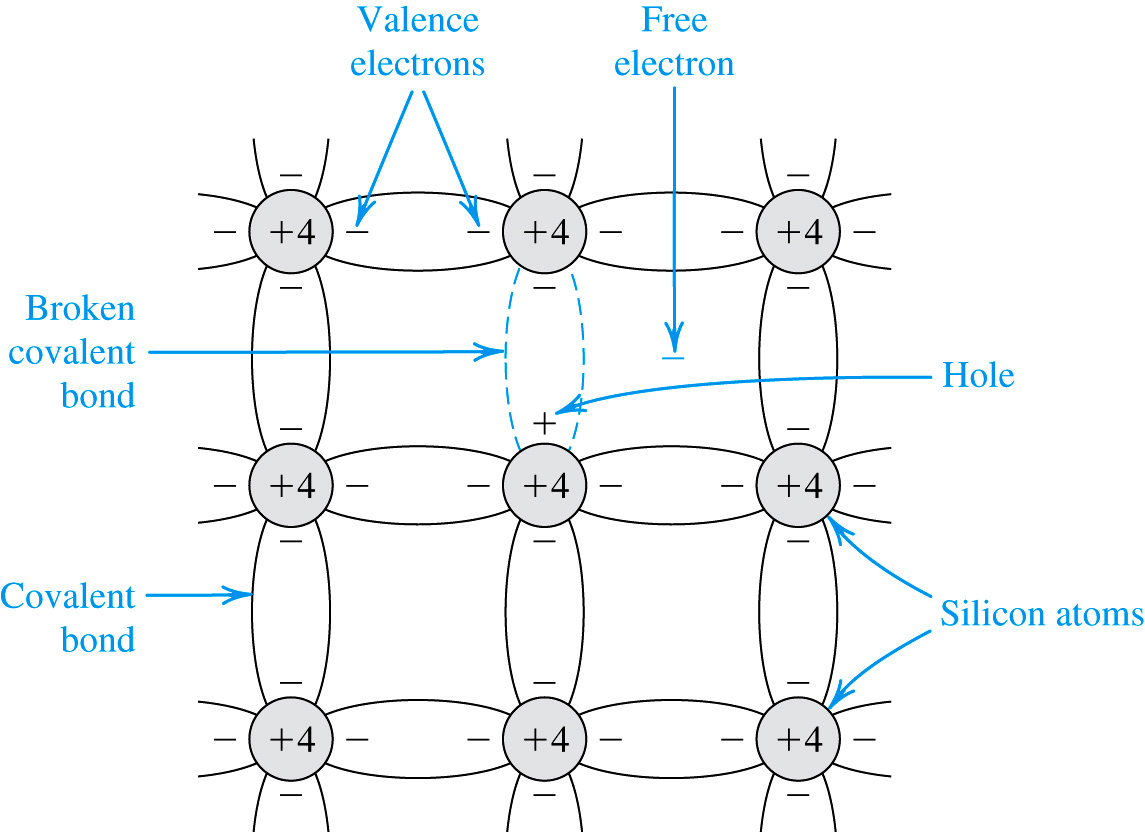
\includegraphics[width=.9\linewidth]{../figs/silicio_T300K.jpg}
\end{center}
\end{column}
\end{columns}
\end{frame}

\begin{frame}[plain,label={sec:orga2d11df}]{Recombinación de un par electrón-hueco}
\begin{columns}
\begin{column}{0.7\columnwidth}
\begin{itemize}[<+->]
\item Se producen \alert{encuentros electrón-hueco} que restablecen un enlace con \alert{liberación de energía} (\(E_{g}\)) en forma de calor.

\item Para evitar la recombinación \alert{es preciso dirigir el movimiento} de electrones y huecos mediante un campo eléctrico.
\end{itemize}
\end{column}

\begin{column}{0.6\columnwidth}
\begin{center}
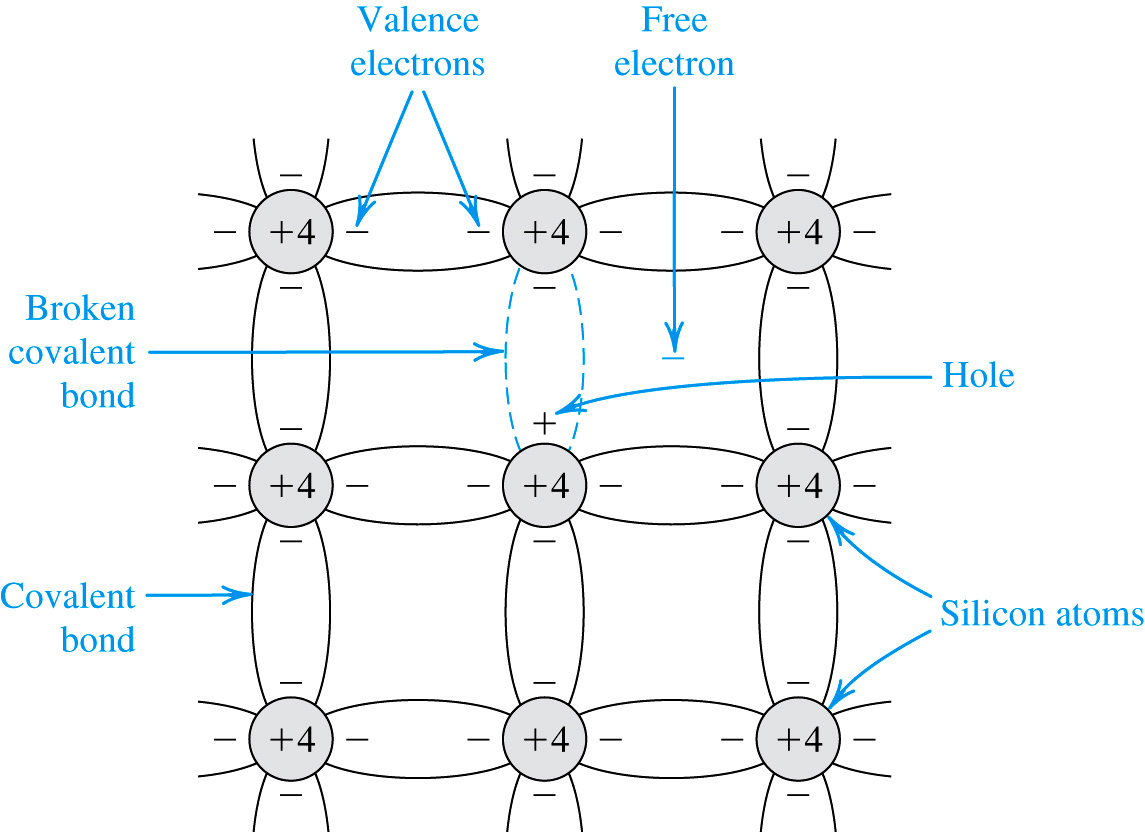
\includegraphics[width=.9\linewidth]{../figs/silicio_T300K.jpg}
\end{center}
\end{column}
\end{columns}
\end{frame}


\subsection{Dopaje de semiconductores}
\label{sec:orge8cd58b}
\begin{frame}[label={sec:org848108a}]{Definición}
El \alert{dopaje de semiconductores} consiste en introducir de forma controlada impurezas en el cristal para alterar las bandas de energía.

\begin{center}
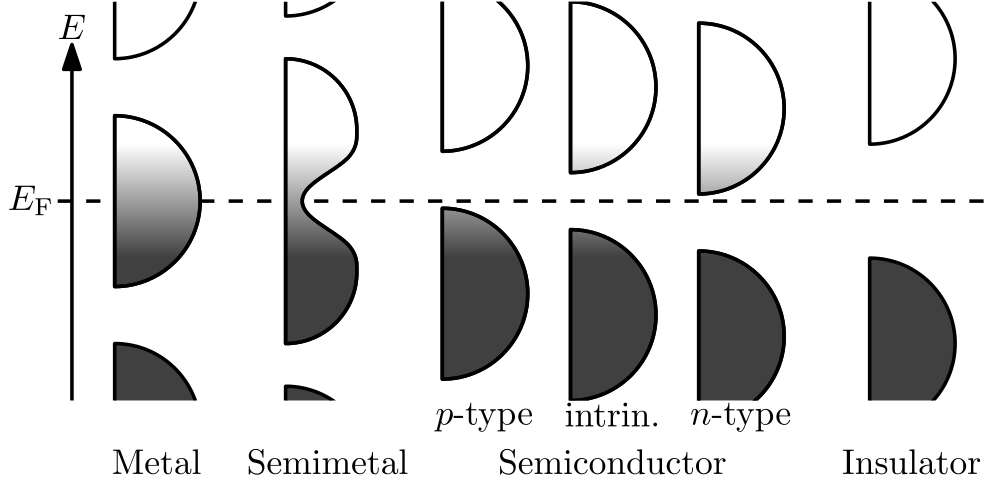
\includegraphics[width=.9\linewidth]{../figs/Band_filling_diagram.png}
\end{center}
\end{frame}

\begin{frame}[label={sec:org37c6e34}]{Tipo n}
\begin{center}
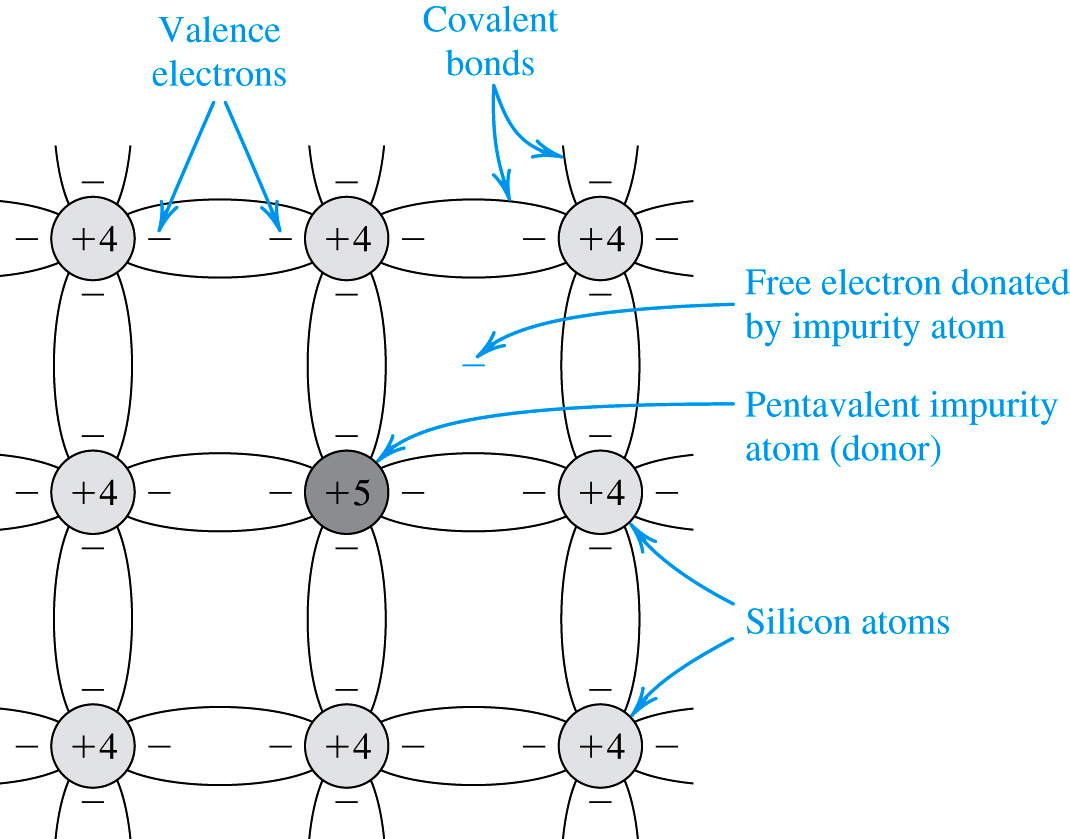
\includegraphics[width=.9\linewidth]{../figs/DopajeN.jpg}
\end{center}

\footnotetext[2]{Figura de Sedra and Smith, Microelectronic Circuits}
\end{frame}
\begin{frame}[plain,label={sec:orgae13508}]{Tipo n}
\begin{columns}
\begin{column}{0.7\columnwidth}
\begin{itemize}[<+->]
\item Los átomos de \alert{Fósforo} tienen cinco electrones de valencia (uno más que el silicio).

\item Al impurificar un cristal de Silicio con átomos de Fósforo, el quinto electrón no queda bien integrado en la red.

\item La rotura de este enlace se produce con \alert{baja aportación energética} (menor que \(E_{g}\)).

\item El \alert{quinto electrón queda libre pero la carga positiva (ión \(P^{+}\)) está ligada} a la red cristalina.

\item La \alert{densidad de electrones} (portador mayoritario) es \alert{superior a la de huecos}
\end{itemize}
\end{column}

\begin{column}{0.5\columnwidth}
\begin{center}
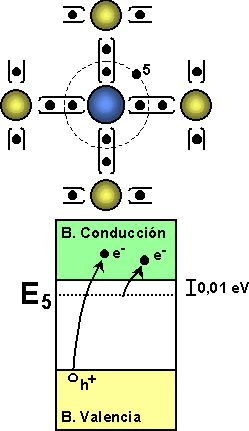
\includegraphics[width=.9\linewidth]{../figs/Semiconductor_tipo_n_vertical.png}
\end{center}
\end{column}
\end{columns}
\end{frame}

\begin{frame}[label={sec:org7e11ea3}]{Tipo p}
\begin{center}
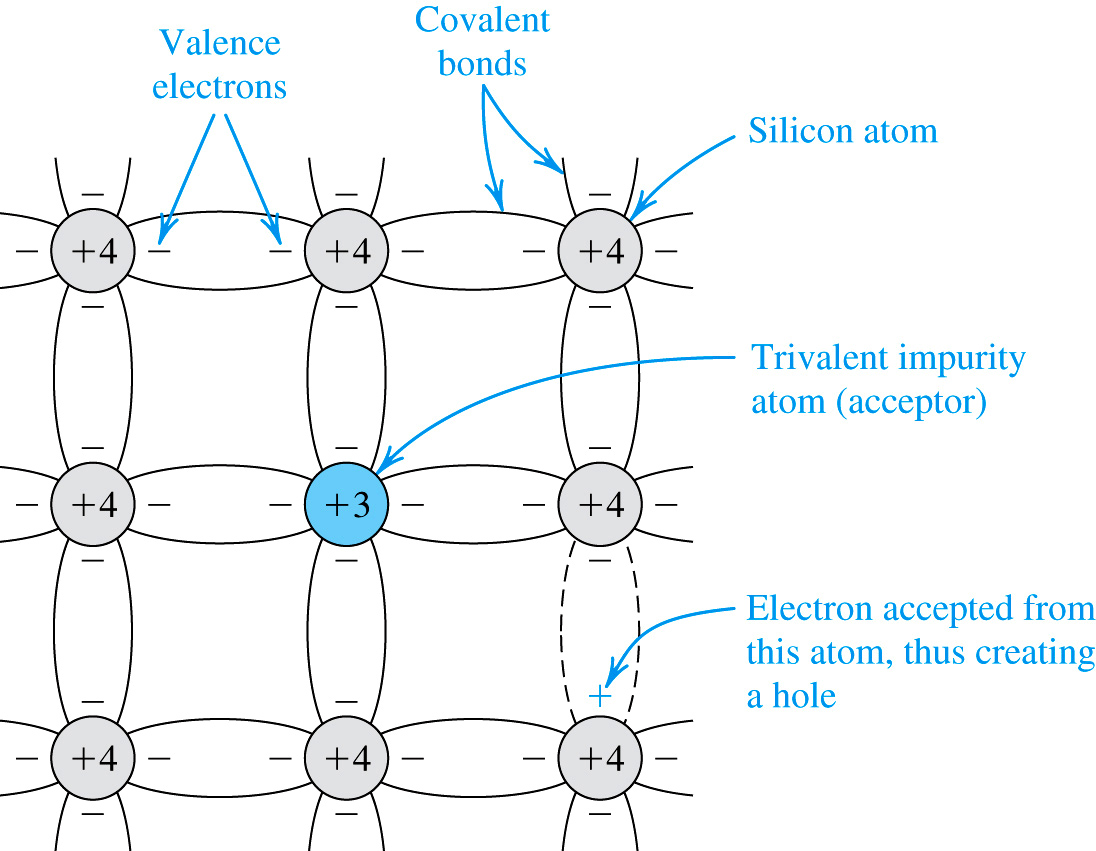
\includegraphics[width=.9\linewidth]{../figs/DopajeP.jpg}
\end{center}

\footnotetext[2]{Figura de Sedra and Smith, Microelectronic Circuits}
\end{frame}
\begin{frame}[plain,label={sec:org4db5ed9}]{Tipo p}
\begin{columns}
\begin{column}{0.7\columnwidth}
\begin{itemize}[<+->]
\item Los átomos de \alert{Boro} tienen tres electrones de valencia (uno menos que el silicio).

\item Al impurificar un cristal de Silicio con átomos de Boro, hay un enlace sin cubrir (hueco).

\item La rotura de este enlace se produce con \alert{baja aportación energética} (menor que \(E_{g}\)).

\item El \alert{hueco queda libre} pero la \alert{carga negativa (ión \(B^{-}\)) está ligada} a la red cristalina.

\item La \alert{densidad de huecos} (portador mayoritario) es \alert{superior a la de electrones}
\end{itemize}
\end{column}
\begin{column}{0.5\columnwidth}
\begin{center}
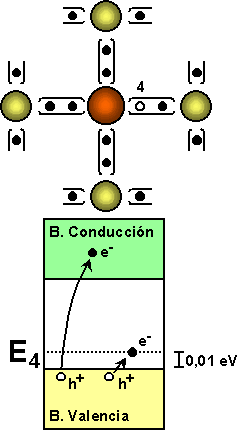
\includegraphics[width=.9\linewidth]{../figs/Semiconductor_tipo_p_vertical.png}
\end{center}
\end{column}
\end{columns}
\end{frame}


\subsection{Unión p-n}
\label{sec:orga7d746a}
\begin{frame}[label={sec:org006ce7a}]{Unión p-n}
\begin{center}
\begin{center}
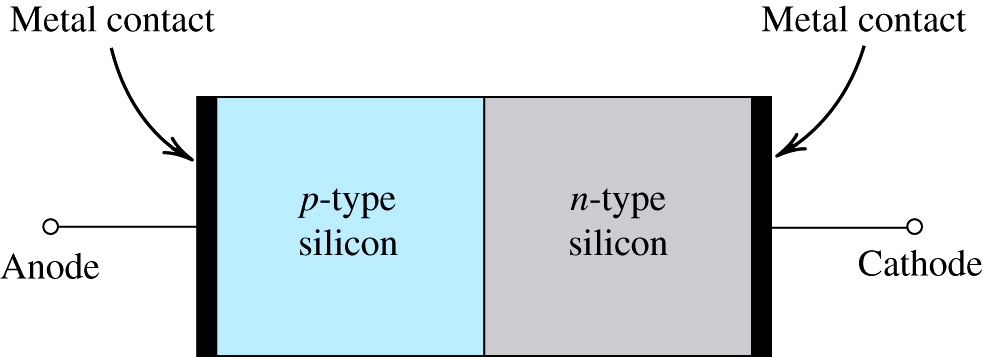
\includegraphics[width=.9\linewidth]{../figs/Union_PN.jpg}
\end{center}
\end{center}

\footnotetext[2]{Figura de Sedra and Smith, Microelectronic Circuits}
\end{frame}

\begin{frame}[label={sec:org0dcdbff}]{Conducción en una unión p-n}
\begin{itemize}
\item Al \alert{unir un semiconductor tipo p con otro tipo n, se produce un desequilibrio}:
\begin{itemize}
\item Corriente de Difusión
\item Corriente de Arrastre
\end{itemize}
\end{itemize}

\begin{center}
\begin{center}
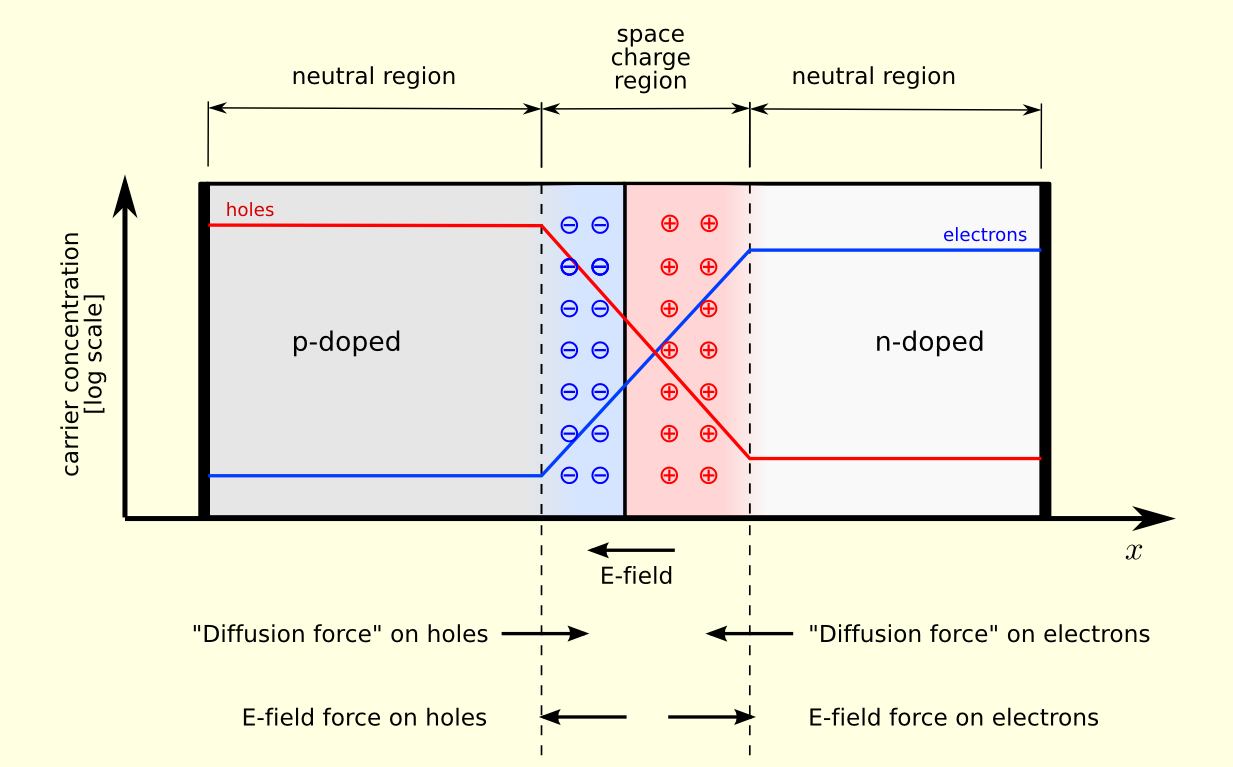
\includegraphics[width=.9\linewidth]{../figs/Pn-junction-equilibrium.png}
\end{center}
\end{center}
\footnotetext[2]{Figura de Sedra and Smith, Microelectronic Circuits}
\end{frame}
\begin{frame}[label={sec:orgc4066f3}]{Corriente de Difusión}
\begin{itemize}
\item \alert{Difusión de portadores mayoritarios}
\begin{itemize}[<+->]
\item Movimiento de huecos desde cristal p a cristal n, dejando iones con carga negativa.

\item Movimiento de electrones desde cristal n a cristal p, dejando iones con carga positiva.
\end{itemize}
\end{itemize}

\begin{center}
\begin{center}
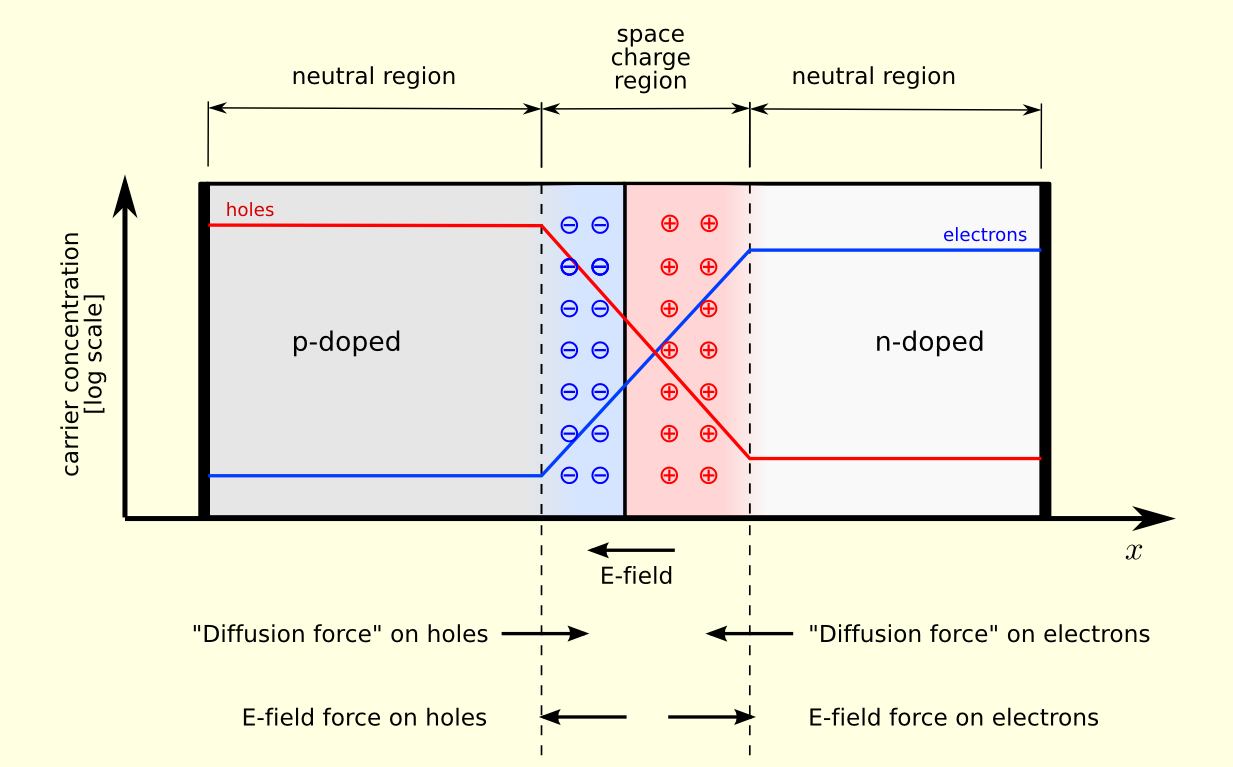
\includegraphics[height=0.5\textheight]{../figs/Pn-junction-equilibrium.png}
\end{center}
\end{center}
\end{frame}

\begin{frame}[label={sec:org7b8d7ca}]{Corriente de Arrastre}
\begin{itemize}[<+->]
\item \alert{Los iones fijos} cercanos a la unión generan un \alert{campo eléctrico de arrastre} en sentido opuesto a la difusión: \alert{barrera de potencial}

\item Los \alert{portadores minoritarios que atraviesan la unión se recombinan} en la \alert{zona cercana a la unión} despoblada de portadores y con iones cargados ligados a la red.
\end{itemize}

\begin{center}
\begin{center}
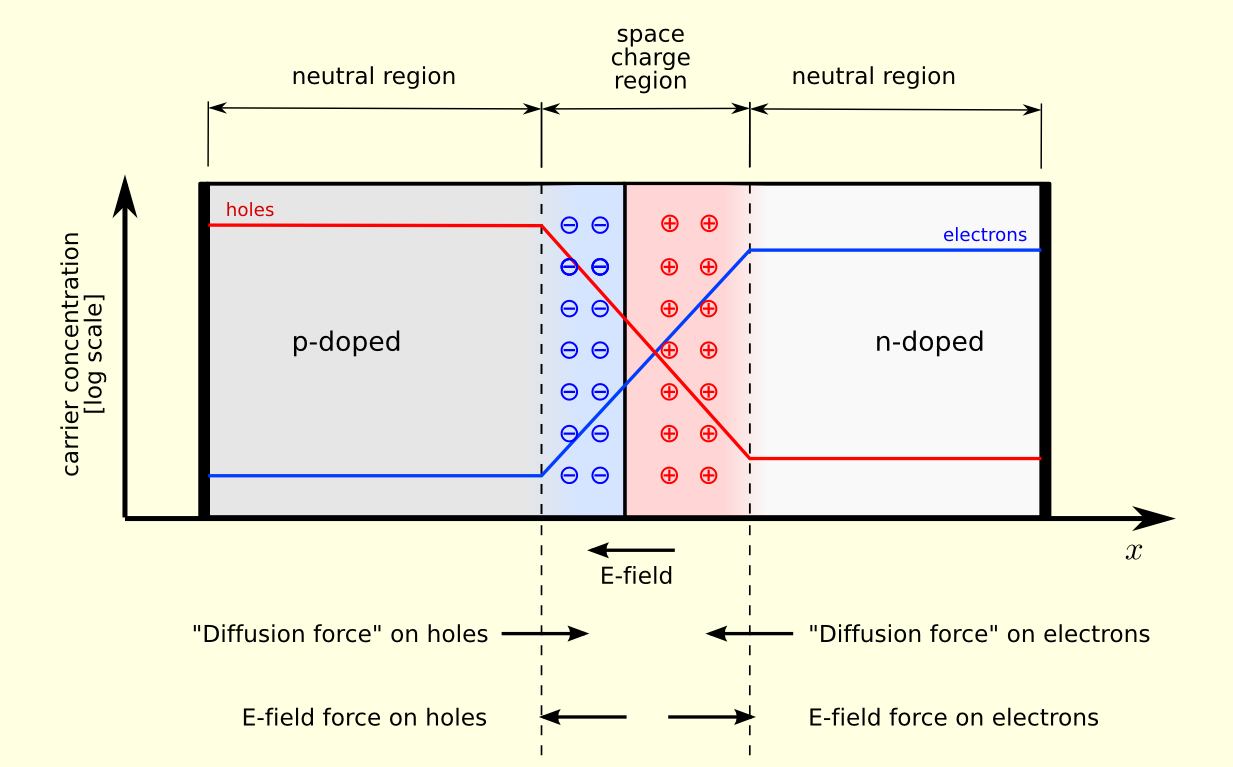
\includegraphics[height=0.5\textheight]{../figs/Pn-junction-equilibrium.png}
\end{center}
\end{center}
\end{frame}


\begin{frame}[label={sec:org4632eef}]{Equilibrio en una unión p-n}
\begin{itemize}
\item El \alert{equilibrio} se alcanza al \alert{compensarse los movimientos de  difusión y de arrastre}.
\end{itemize}

\begin{center}
\begin{center}
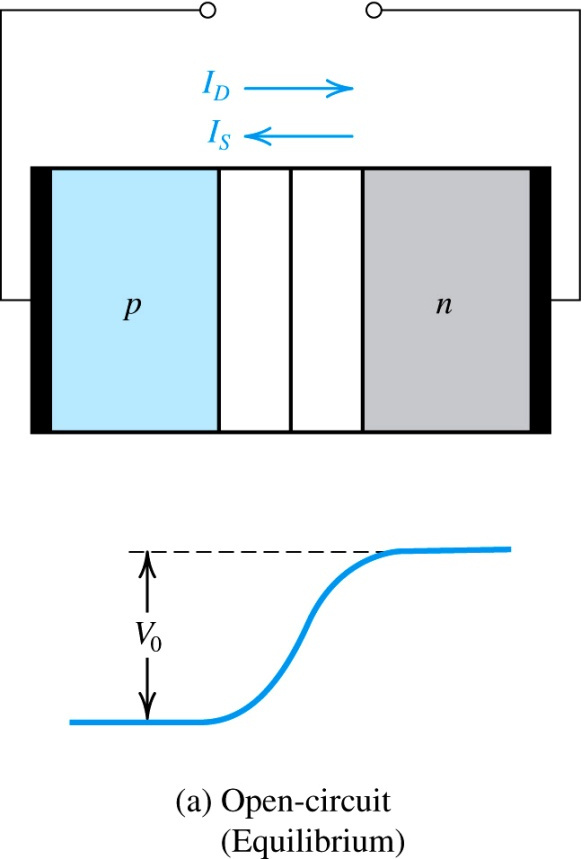
\includegraphics[height=0.5\textheight]{../figs/Diodo_CircuitoAbierto.jpg}
\end{center}
\end{center}
\footnotetext[2]{Figura de Sedra and Smith, Microelectronic Circuits}
\end{frame}

\begin{frame}[plain,label={sec:orgde0bf29}]{Polarización en directa}
\begin{columns}
\begin{column}{0.7\columnwidth}
\begin{itemize}[<+->]
\item Para \alert{conseguir corriente} es necesario \alert{romper el equilibrio} alcanzado y \alert{reducir la barrera de potencial}.

\item Diferencia de potencial con lado \alert{p positivo respecto al lado n}: unión p-n está polarizada en directa.

\item En estas condiciones \alert{se reduce la barrera de potencial} y, en consecuencia el valor del campo eléctrico de la zona de unión.

\item La \alert{corriente de arrastre disminuye} y \alert{no puede compensar la corriente de difusión}.

\item Convenio: la corriente entra por zona p y sale por zona n.
\end{itemize}
\end{column}
\begin{column}{0.5\columnwidth}
\begin{center}
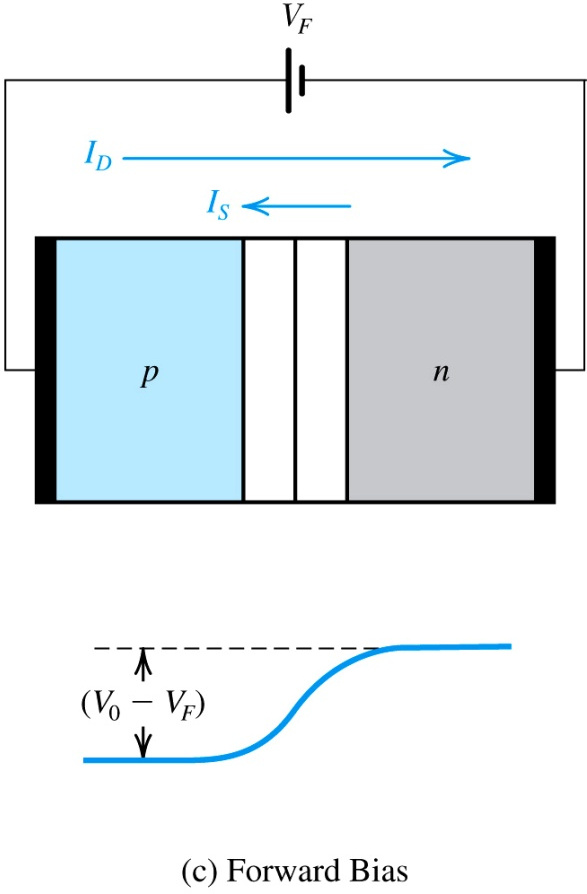
\includegraphics[width=.9\linewidth]{../figs/Diodo_Directa.jpg}
\end{center}
\end{column}
\end{columns}
\end{frame}

\begin{frame}[plain,label={sec:org04cb126}]{Polarización en inversa}
\begin{columns}
\begin{column}{0.7\columnwidth}
\begin{itemize}[<+->]
\item Si la diferencia de potencial aplicada consigue que la \alert{zona p esté a menor tensión que la zona n}, la unión queda polarizada en inversa.

\item En estas condiciones \alert{la barrera de potencial en la unión queda reforzada} y el paso de portadores de una a otra zona queda aún más debilitado.

\item La \alert{corriente que atraviesa la unión en polarización inversa es de muy bajo valor}.
\end{itemize}
\end{column}

\begin{column}{0.5\columnwidth}
\begin{center}
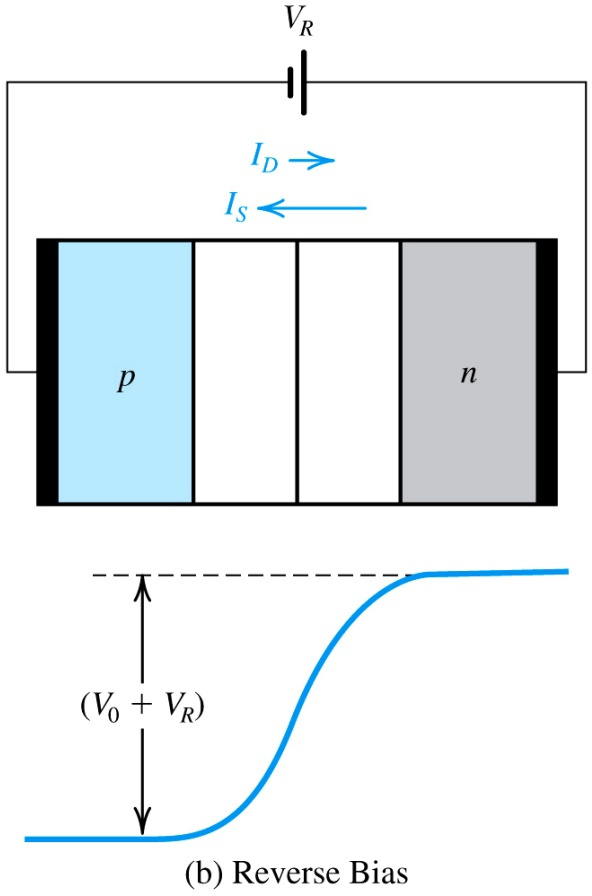
\includegraphics[width=.9\linewidth]{../figs/Diodo_Inversa.jpg}
\end{center}
\end{column}
\end{columns}
\end{frame}


\subsection{Diodo}
\label{sec:org1ab3e58}

\begin{frame}[label={sec:org751e45b}]{Definición}
\begin{itemize}
\item El dispositivo electrónico basado en una unión p-n se denomina diodo.

\item La zona p del diodo es el ánodo y la zona n es el cátodo.
\end{itemize}
\begin{center}
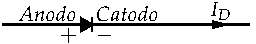
\includegraphics[width=0.5\textwidth]{../figs/Diodo.pdf}
\end{center}
\end{frame}

\begin{frame}[label={sec:orgbdb0242}]{Ecuación del Diodo}
\begin{itemize}
\item $$I_{D}=I_{0}\cdot[\exp(\frac{V}{m\cdot V_{T}})-1]$$ donde \(I_{0}\) es la corriente de saturación en oscuridad del diodo, \(V\) la tensión aplicada al diodo y \(m\) el factor de idealidad del diodo.

\item Para una temperatura ambiente de \(\SI{300}{\kelvin}\),
\end{itemize}
$$V_{T}=\frac{\mathrm{k}T}{\mathrm{e}}=\SI{25.85}{\milli\volt}$$ donde
\(\mathrm{k}\) es la constante de Boltzmann, \(T\) la temperatura del diodo
(en grados Kelvin), y \(\mathrm{e}\) es la carga del electrón.
\end{frame}

\begin{frame}[label={sec:org067dd21}]{}
\begin{center}
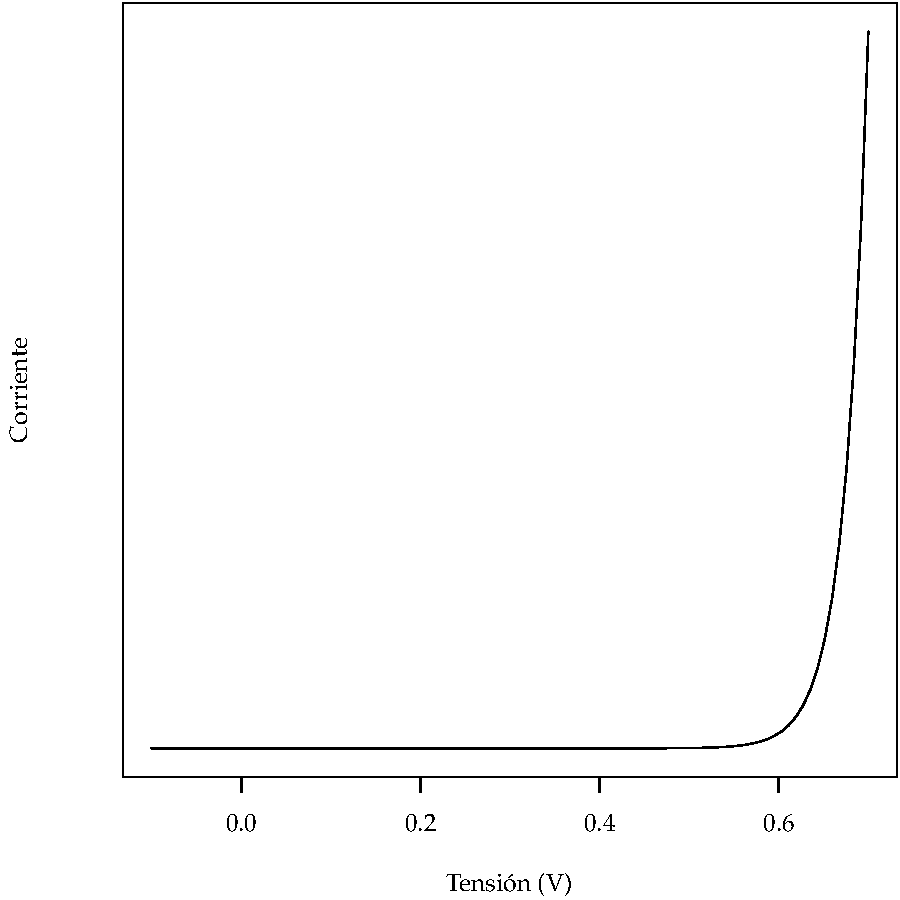
\includegraphics[width=.9\linewidth]{../figs/EcuacionDiodo.pdf}
\end{center}
\end{frame}


\section{Unión P-N iluminada}
\label{sec:org6022a90}

\begin{frame}[label={sec:org8284dfb}]{}
\begin{center}
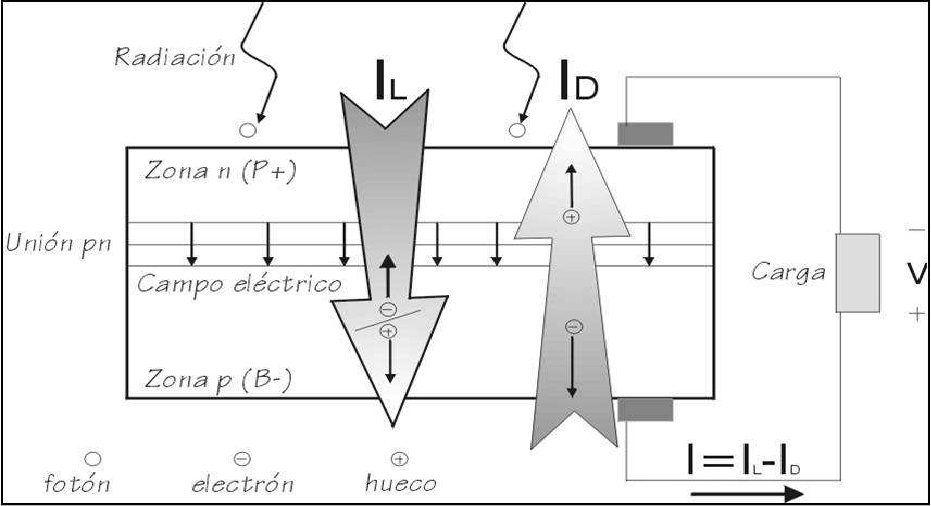
\includegraphics[width=.9\linewidth]{../figs/CelulaSolar.pdf}
\end{center}
\end{frame}

\begin{frame}[label={sec:org2ec7c83}]{Efecto fotoeléctrico}
\begin{itemize}[<+->]
\item Efecto fotoeléctrico: \alert{los electrones se desplazan a la banda de conducción por el aporte energético de fotones} (\(E_{f}=\frac{h\cdot c}{\lambda}\)).

\item Al \alert{iluminar una unión p-n}, el \alert{campo eléctrico} de la unión conduce los portadores y \alert{dificulta la recombinación}.

\item La \alert{fotocorriente} es ahora \alert{aprovechable} por un circuito externo (\emph{corriente de iluminación, corriente de generación})

\item La presencia de \alert{tensión en los terminales} de la unión (por ejemplo, caída de tensión en una resistencia alimentada por la fotocorriente) \alert{favorece la recombinación} (\emph{corriente de oscuridad o corriente de diodo}).
\end{itemize}
\end{frame}


\begin{frame}[label={sec:orgbadae5e}]{Absorción de luz y generación de portadores}
\begin{itemize}[<+->]
\item Si el \alert{fotón es poco energético} (\(E_{f}<E_{g}\)) \alert{no interactúa con
el semiconductor} (como si fuese transparente)

\begin{itemize}
\item Fotones en el espectro visible (\(400\, nm<\lambda<700\, nm\)) y
ultravioleta (\(\lambda<400\, nm\)) rompen enlaces.

\item Si \(\lambda>1100\, nm\) (infrarrojo) el fotón no interactúa.
\end{itemize}

\item Los \alert{fotones más energéticos} (baja longitud de onda) son \alert{absorbidos en la superficie}.

\item Los \alert{fotones menos energéticos} (alta longitud de onda) penetran en el interior hasta \alert{romper un enlace}.
\end{itemize}
\end{frame}

\begin{frame}[label={sec:orgf9c5114}]{Absorción de luz y generación de portadores}
\begin{itemize}[<+->]
\item Los fotones con \(E_{f}<E_{g}\) atraviesan el cristal sin ser absorbidos: \alert{pérdidas de no-absorción}

\item Fotones con \(E_{f}>E_{g}\):

\begin{itemize}
\item Debido a anchura del semiconductor y coeficiente de absorción del
material parte no son absorbidos: \alert{pérdidas de transmisión}

\item Debido a diferencia de índices de refracción: \alert{pérdidas de
reflexión}

\item Parte de los portadores generadores se recombinan dentro del
dispositivo: \alert{pérdidas por recombinación}
\end{itemize}
\end{itemize}
\end{frame}

\section{Funcionamiento de una célula solar}
\label{sec:org75cc2f7}

\begin{frame}[label={sec:orgaa96a88}]{}
\begin{center}
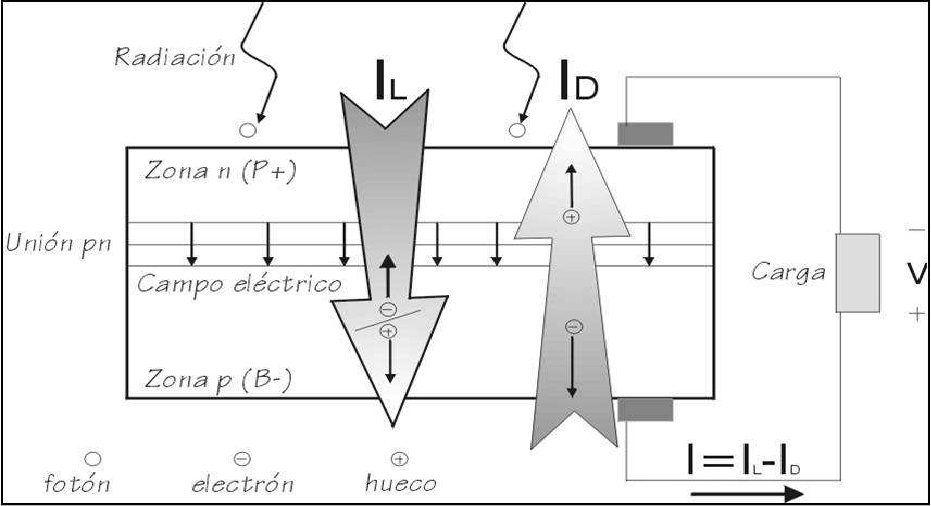
\includegraphics[width=.9\linewidth]{../figs/CelulaSolar.pdf}
\end{center}
\end{frame}


\subsection{Curva IV y Puntos Característicos}
\label{sec:org54654af}
\begin{frame}[label={sec:org0ed13ca}]{Característica I-V de iluminación}
$$I=I_{L}-I_{D}$$

$$I_{D}=I_{0}\cdot\left[\exp\left(\frac{e\cdot V}{m\cdot k\cdot
      T_{c}}\right)-1\right]$$

\begin{center}
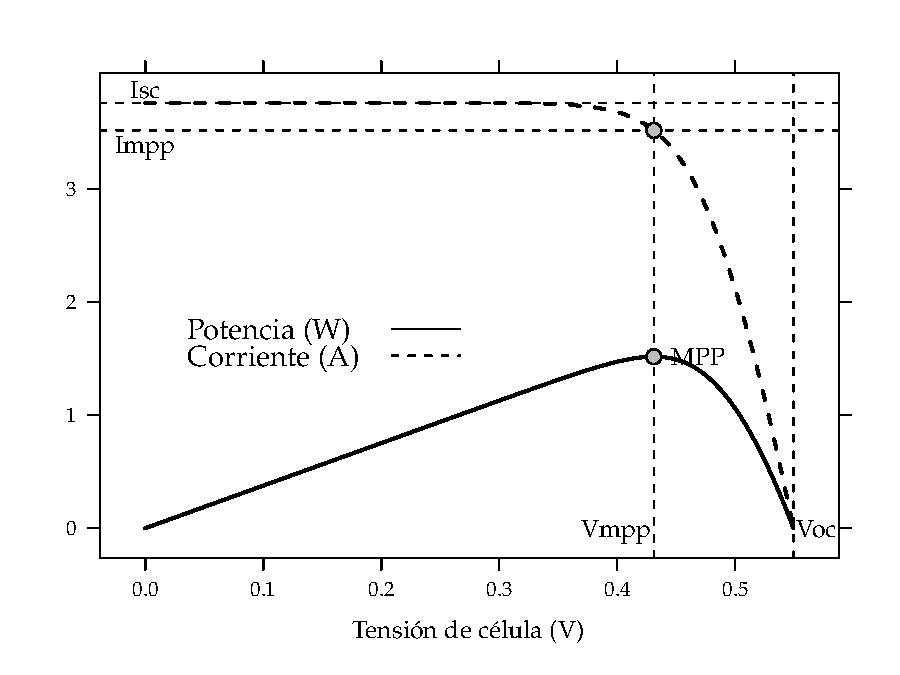
\includegraphics[width=.9\linewidth]{../figs/CurvaIV_Ta20_G800.pdf}
\end{center}
\end{frame}

\begin{frame}[label={sec:org88ea742}]{Isc y Voc}
\begin{block}{Corriente de Cortocircuito}
$$I_{sc}=I(V=0)\Rightarrow I_{D}=0\Rightarrow I=I_{L}$$
\end{block}

\begin{block}{Tensión de Circuito Abierto}
$$V_{oc}=V(I=0)\Rightarrow I_{L}=I_{D}\Rightarrow
V_{oc}=m\cdot\frac{k\cdot
  T_{c}}{e}\cdot\ln\left(\frac{I_{L}}{I_{0}}+1\right)$$
\end{block}

\begin{block}{Ecuación general}
$$I=I_{sc}\cdot\left[1-\exp\left(\frac{e\cdot(V_{oc}-V)}{m\cdot k\cdot
      T_{c}}\right)\right]$$
\end{block}
\end{frame}


\begin{frame}[label={sec:orgb5d3f9c}]{Punto de máxima potencia}
\begin{block}{\(0<V<V_{mpp}\)}
\[
\frac{dP}{dV}>0 \Rightarrow \frac{dI}{dV}>-\frac{I}{V}
\]

\begin{center}
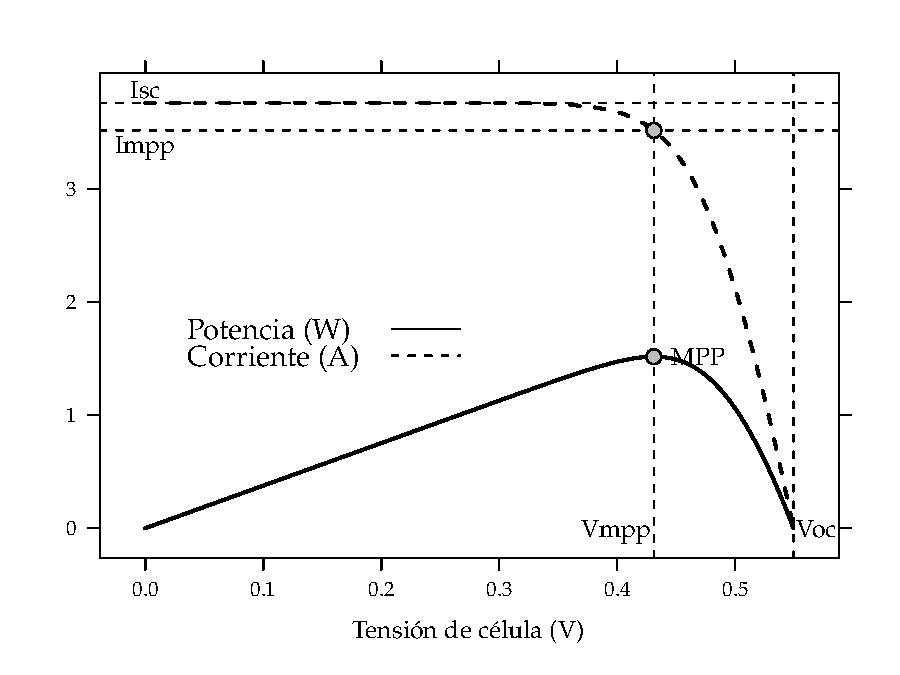
\includegraphics[height=0.65\textheight]{../figs/CurvaIV_Ta20_G800.pdf}
\end{center}
\end{block}
\end{frame}

\begin{frame}[label={sec:orgccabbe3}]{Punto de máxima potencia}
\begin{block}{V=V\(_{\text{mpp}}\)}
\[
\frac{dP}{dV}=0 \Rightarrow \frac{dI}{dV}=-\frac{I}{V}
\]

\begin{center}
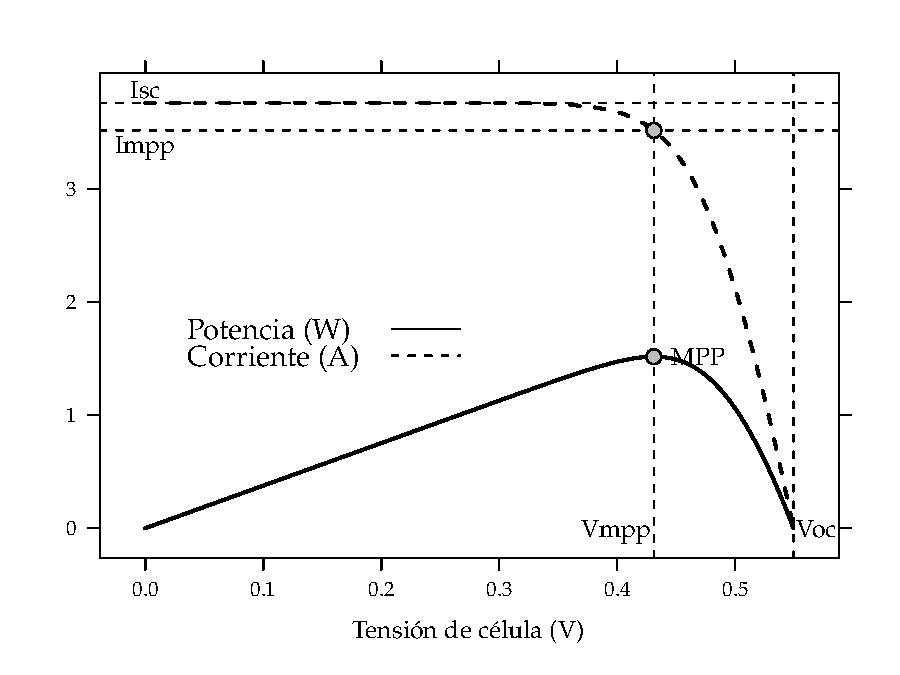
\includegraphics[height=0.65\textheight]{../figs/CurvaIV_Ta20_G800.pdf}
\end{center}
\end{block}
\end{frame}

\begin{frame}[label={sec:org17811dd}]{Punto de máxima potencia}
\begin{block}{\(V_{mpp}<V<V_{oc}\)}
\[
\frac{dP}{dV}<0 \Rightarrow \frac{dI}{dV}<-\frac{I}{V}
\]

\begin{center}
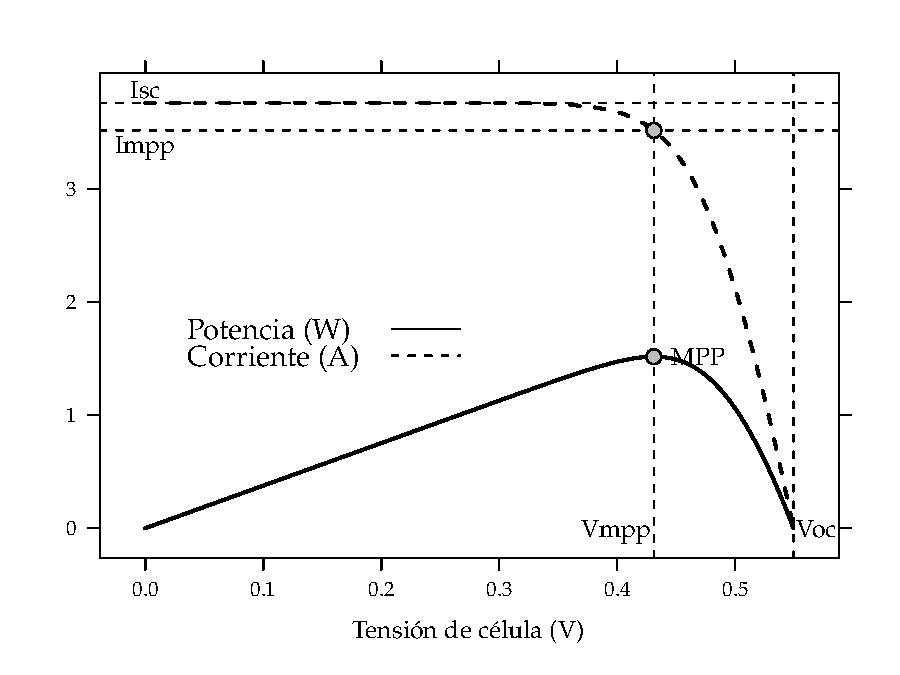
\includegraphics[height=0.65\textheight]{../figs/CurvaIV_Ta20_G800.pdf}
\end{center}
\end{block}
\end{frame}


\begin{frame}[label={sec:orgfa7e367}]{Factor de forma y Eficiencia}
\begin{itemize}
\item Factor de Forma
\end{itemize}
$$FF=\frac{I_{mpp}\cdot V_{mpp}}{I_{sc}\cdot V_{oc}}$$

$$P_{mpp}=FF\cdot I_{sc}\cdot V_{oc}$$

\begin{itemize}
\item Eficiencia
\end{itemize}

$$\eta = \frac{I_{mpp}\cdot V_{mpp}}{P_{L}}$$
$$\eta = \frac{I_{mpp}\cdot V_{mpp}}{A \cdot G}$$
\end{frame}

\begin{frame}[plain,label={sec:org35c238c}]{Eficiencia de células}
\begin{center}
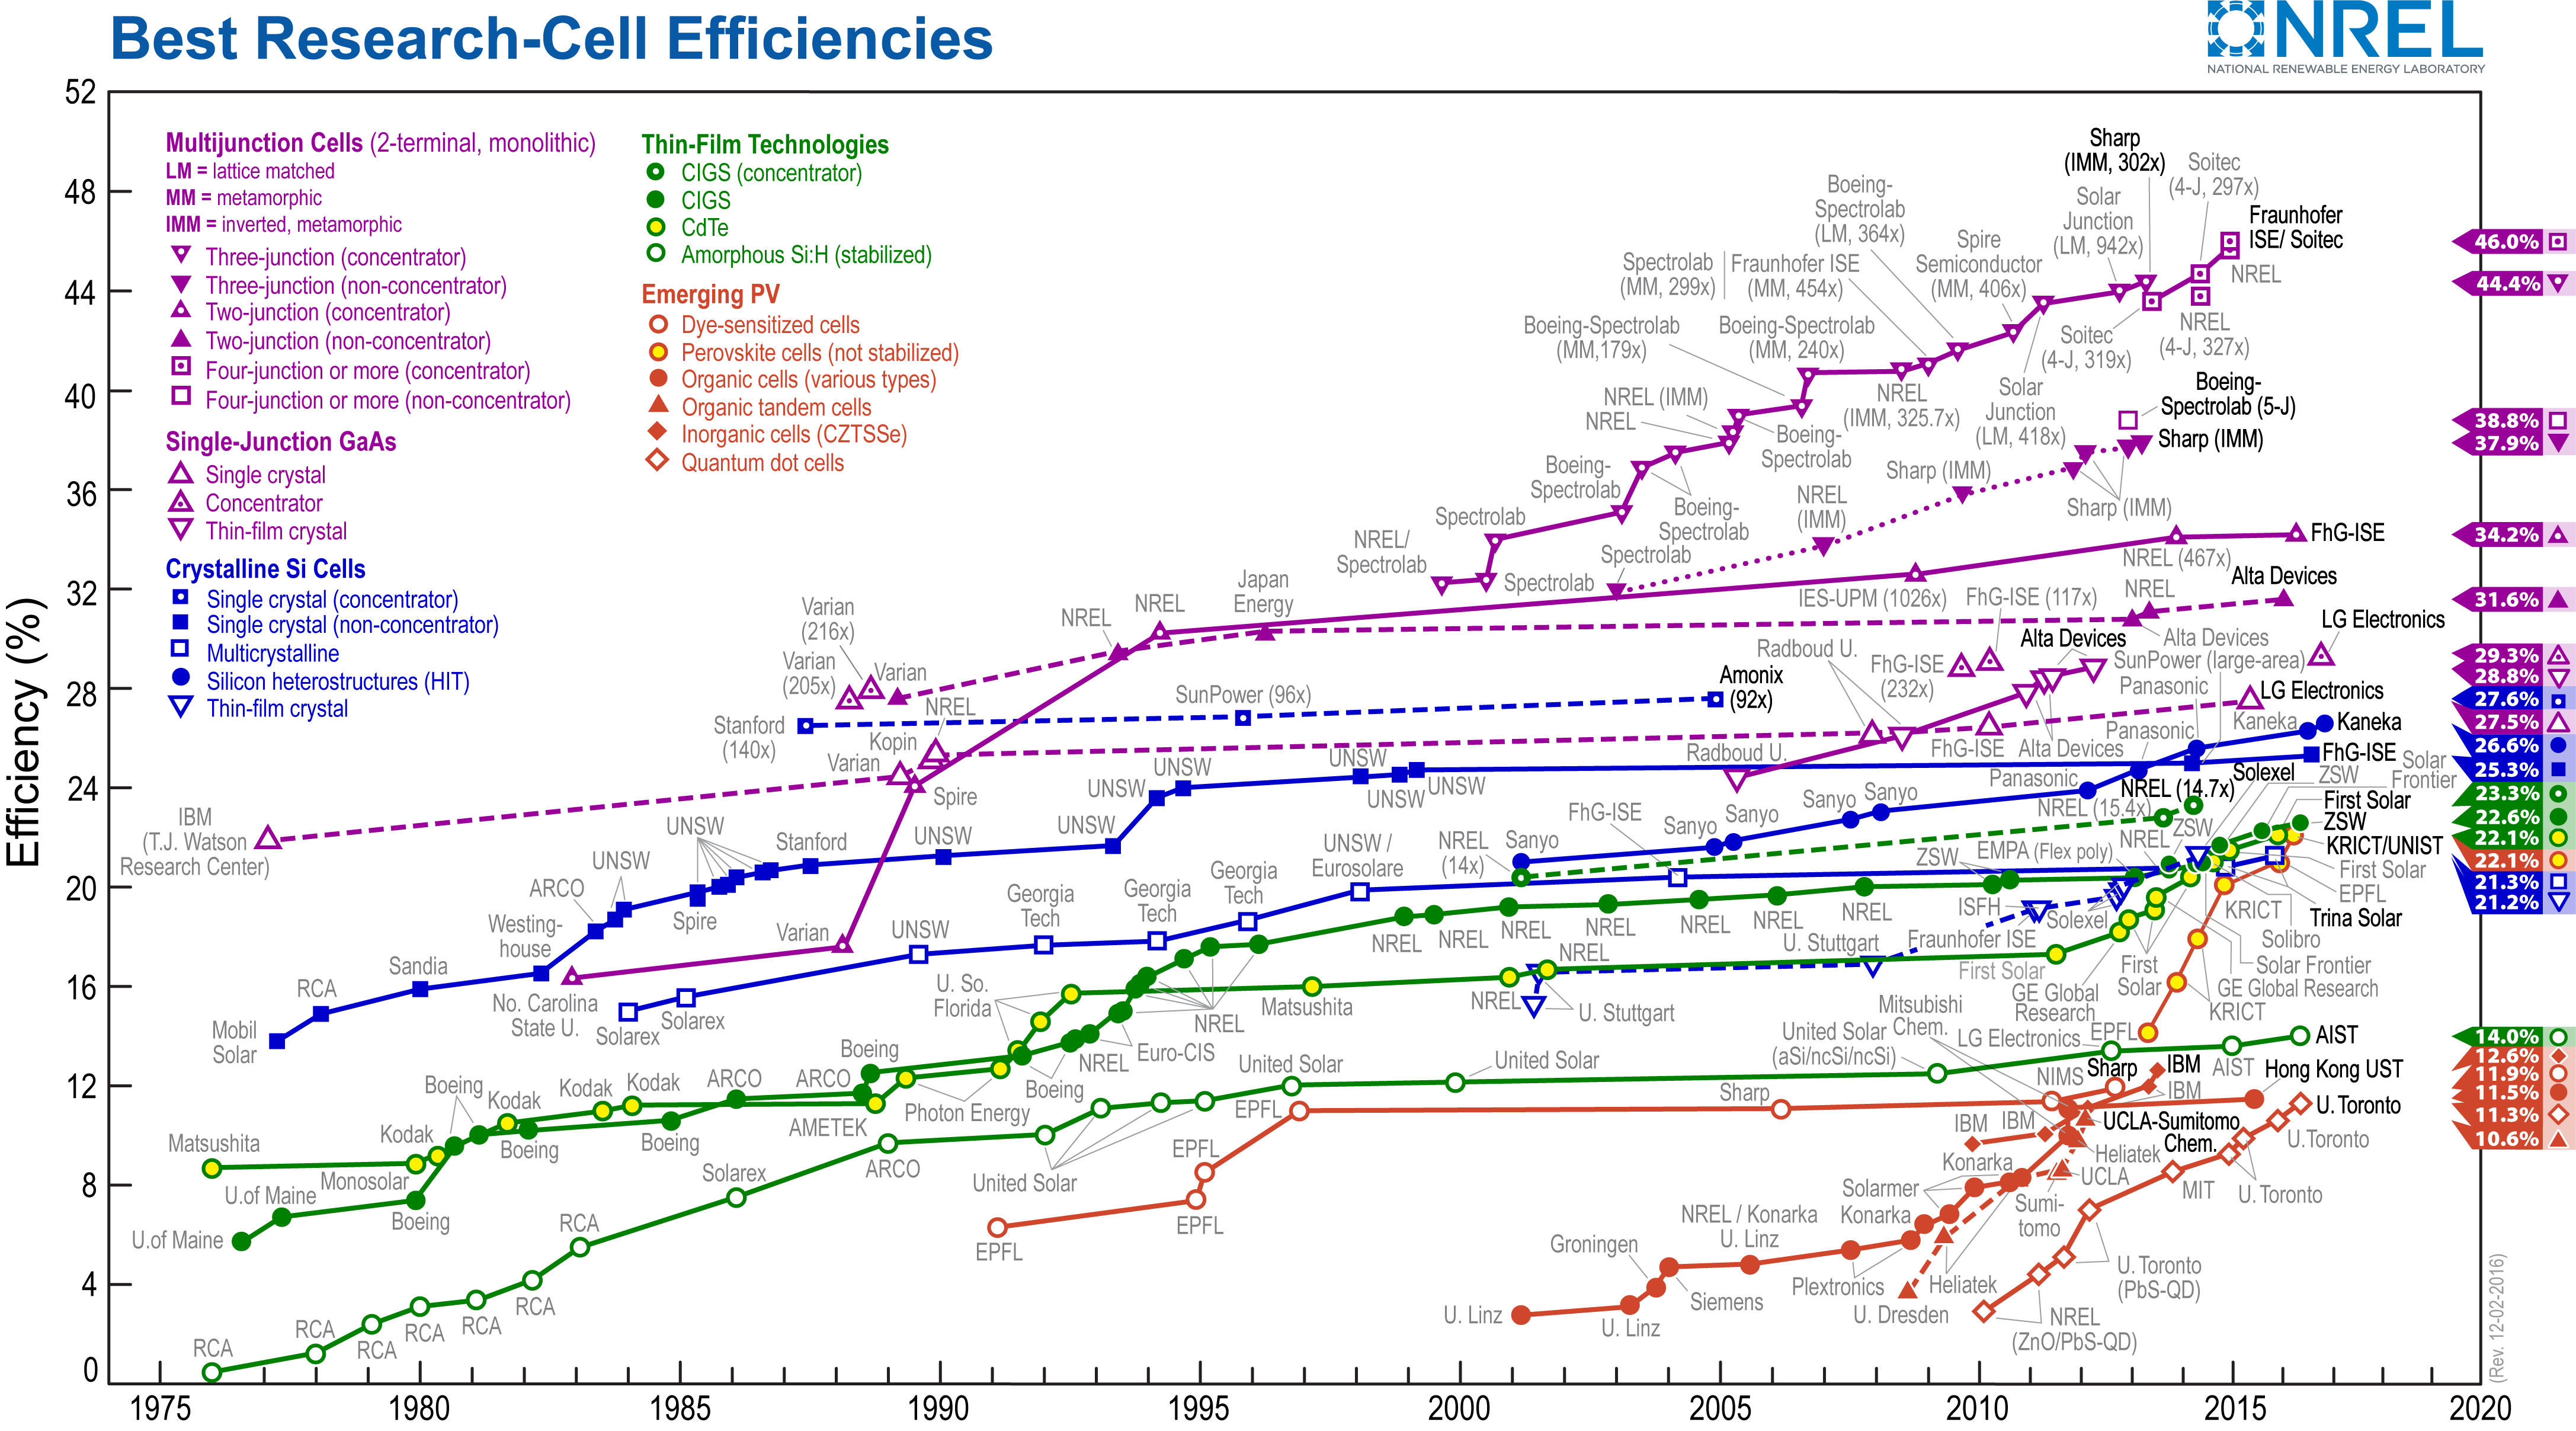
\includegraphics[width=1.2\textwidth]{../figs/efficiency_chart_nrel.jpg}
\end{center}

\url{http://www.nrel.gov/ncpv/}
\end{frame}

\subsection{Influencia de Temperatura y Radiación}
\label{sec:orgd53cfde}

\begin{frame}[label={sec:org58f0aec}]{Radiación}
\begin{itemize}
\item \alert{Corriente de cortocircuito proporcional a intensidad de radiación}
\(I_{sc} = I^*_{sc}\cdot\frac{G_{ef}}{G^{*}}\)

\item Relación logarítmica con tensión de circuito abierto:
\(V_{oc2}=V_{oc1}+\frac{mkT}{e}\cdot\ln(G_2/G_1)\)

\item El factor de forma aumenta ligeramente

\item La eficiencia crece de forma logarítmica hasta determinado nivel.
\end{itemize}
\end{frame}

\begin{frame}[label={sec:org7ed3f6e}]{Influencia de la Radiación}
\begin{center}
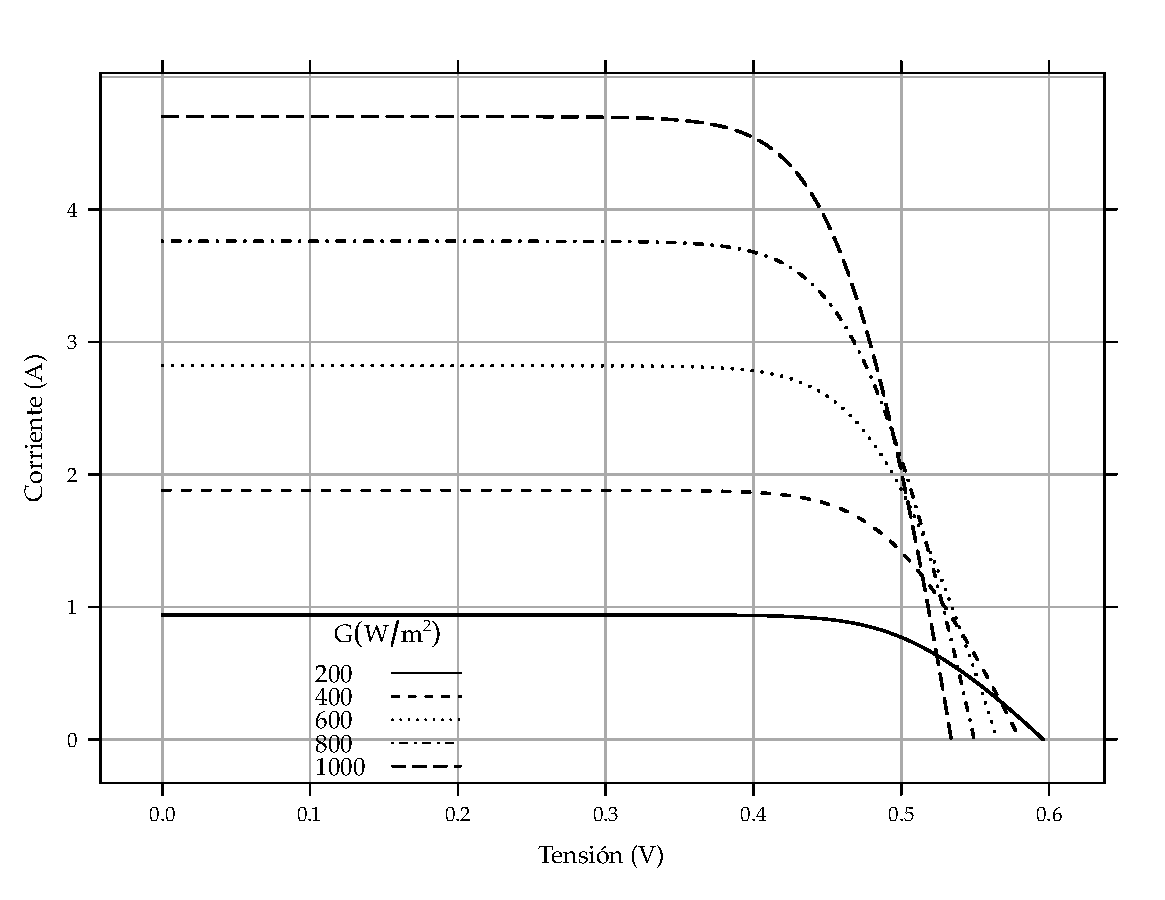
\includegraphics[width=.9\linewidth]{../figs/CurvaIV_Ta20.pdf}
\end{center}
\end{frame}

\begin{frame}[label={sec:orgad1471e}]{Temperatura}
\begin{itemize}
\item Se estrecha el salto entre banda de valencia y conducción: aumenta \emph{ligeramente} la fotocorriente

\item \alert{Disminuye linealmente la tensión de circuito abierto}: \(dV_{oc}/dT_{c}=\SI{-2.3}{\milli\volt\per\celsius}\)

\item Disminuye el factor de forma y la eficiencia:
\(d\eta/dT_{c}=\SI{-0.4}{\percent\per\celsius}\)
\end{itemize}
\end{frame}

\begin{frame}[label={sec:org87cc18a}]{Influencia de la Temperatura}
\begin{center}
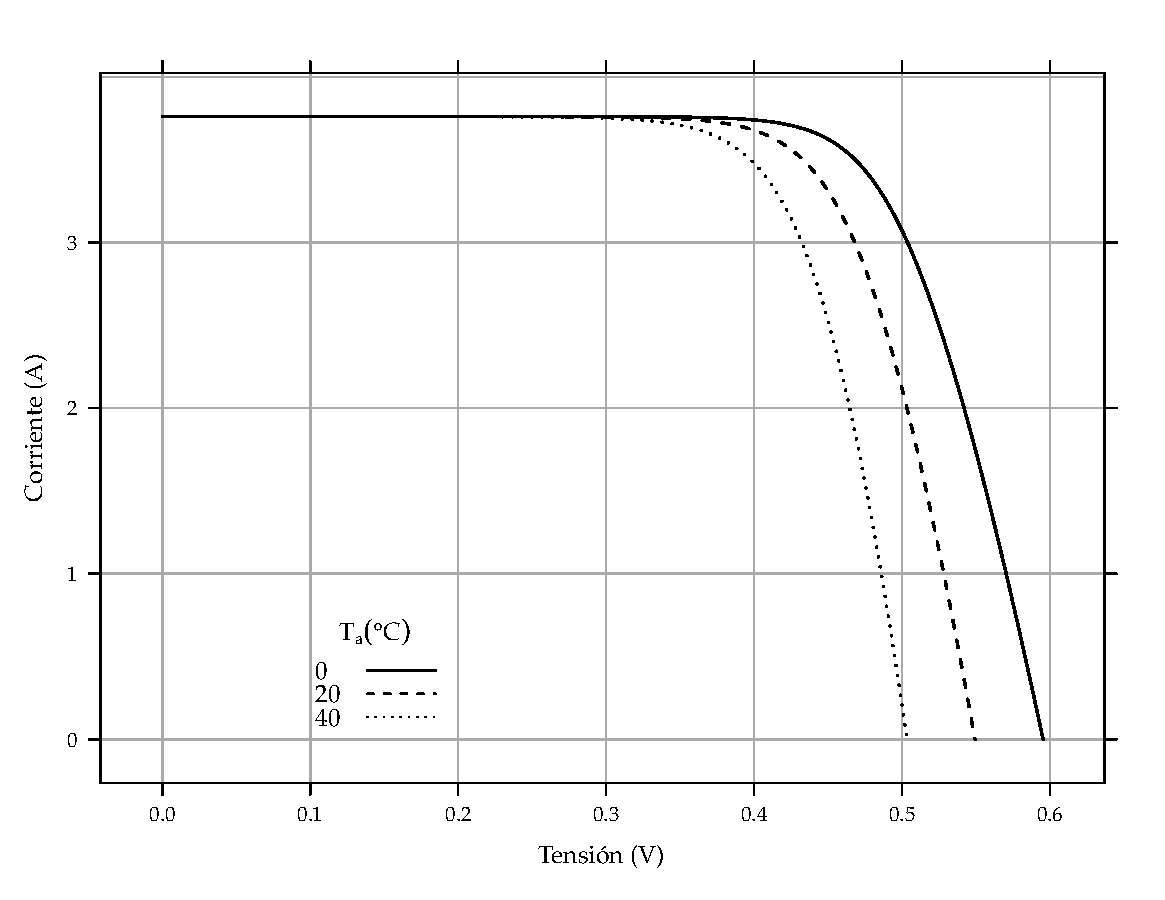
\includegraphics[width=.9\linewidth]{../figs/CurvaIV_G800.pdf}
\end{center}
\end{frame}

\begin{frame}[label={sec:orgdd8e8ac}]{Condiciones Estándar de Medida}
\begin{itemize}
\item Irradiancia: \(G^{*}=\SI{1000}{\watt\per\meter\squared}\) con
incidencia normal.

\item Temperatura de célula: \(T_{c}^{*}=\SI{25}{\celsius}\).

\item Masa de aire: \(AM=1.5\)
\end{itemize}

$$P_{mpp}^{*}=I_{mpp}^{*}\cdot V_{mpp}^{*}$$

$$\eta^{*}=\frac{I_{mpp}^{*}\cdot V_{mpp}^{*}}{A\cdot G^{*}}$$
\end{frame}


\subsection{Cálculo del MPP}
\label{sec:org6c6f3ab}

\begin{frame}[label={sec:orgb640216}]{Método Simplificado: Factor de Forma Constante}
$$FF=FF^{*}$$

$$\begin{aligned}
  \frac{I_{mpp}}{I_{sc}} & = & \frac{I_{mpp}^{*}}{I_{sc}^{*}}\\
  \frac{V_{mpp}}{V_{oc}} & = & \frac{V_{mpp}^{*}}{V_{oc}^{*}}\end{aligned}$$
\end{frame}

\begin{frame}[label={sec:org64dea33}]{Procedimiento}
\begin{itemize}
\item Calcular \(V_{oc}\) a la temperatura \(T_c\):
\end{itemize}

\[
V_{oc} = V_{oc}^* + \frac{dV_{oc}}{dT_{c}} \cdot (T_c - T^*_c)
\]

\begin{itemize}
\item Calcular \(V_{mpp}\) a la temperatura \(T_c\):
\end{itemize}

\[
V_{mpp} = V_{oc} \cdot \frac{V_{mpp}^*}{V_{oc}^{*}}
\]

\begin{itemize}
\item Calcular \(I_{sc}\) a la radiación \(G_{ef}\).
\end{itemize}

\[
I_{sc} = I_{sc}^* \cdot \frac{G_{ef}}{G^*}
\]

\begin{itemize}
\item Calcular \(I_{mpp}\) a la radiación \(G_{ef}\)
\end{itemize}

\[
I_{mpp} = I_{sc} \cdot \frac{I_{mpp}^{*}}{I_{sc}^{*}}
\]
\end{frame}

\begin{frame}[label={sec:orgc62945c}]{Ejercicio de Cálculo}
De una célula de \(\SI{100}{\centi\meter\squared}\) y \(I_{sc}^{*}=3\, A\), \(I_{mpp}^{*}=2.7\, A\) , \(V_{oc}^{*}=0.6\, V\),
\(V_{mpp}^{*}=0.48\, V\), calcular suponiendo factor de forma constante:

\begin{itemize}
\item \(P_{mpp}^{*}\), \(FF^{*}\), \(\eta^{*}\)

\item \(I_{mpp}\), \(V_{mpp}\) cuando \(T_{c}=60\celsius\) y \(G=800\, W/m^{2}\).
\end{itemize}
\end{frame}


\subsection{Circuito equivalente de la célula}
\label{sec:org5e1869c}

\begin{frame}[label={sec:orgf1e4d45}]{Circuito equivalente}
\begin{center}
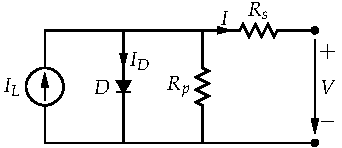
\includegraphics[width=.9\linewidth]{../figs/ModeloElectricoCelulaSolar.pdf}
\end{center}

\begin{itemize}
\item Ecuación general
\end{itemize}

\[I=I_{L}-I_{0}\cdot[\exp(\frac{V+I\cdot R_{s}}{m\cdot
  V_{T}})-1]-\frac{V+I\cdot R_{s}}{R_{p}}\]

\begin{itemize}
\item Ecuación simplificada
\end{itemize}

$$I=I_{sc}[1-\exp(\frac{V-V_{oc}+I\cdot R_{s}}{m\cdot V_{t}})]$$
\end{frame}

\begin{frame}[label={sec:org5451d90}]{Resistencia Serie: Curva IV}
\begin{itemize}
\item Resistencia de contactos metálicos con el semiconductor

\item Resistencia de capas semiconductoras

\item Resistencia de malla de metalización
\end{itemize}

\begin{center}
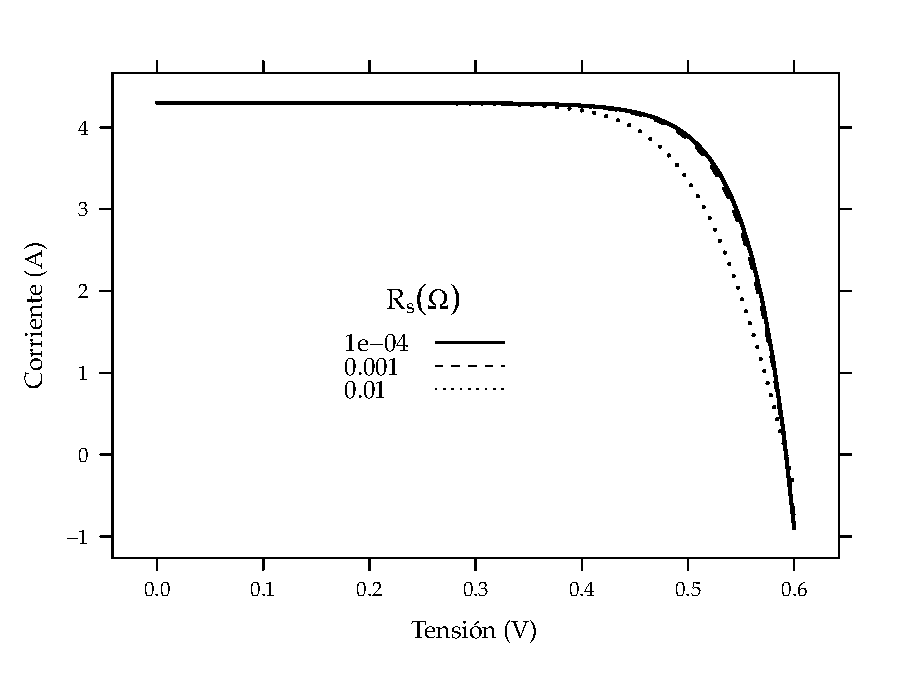
\includegraphics[width=.9\linewidth]{../figs/InfluenciaRs_IV.pdf}
\end{center}
\end{frame}

\begin{frame}[label={sec:org6e34d5f}]{Resistencia Serie: Curva PV}
\begin{itemize}
\item Resistencia de contactos metálicos con el semiconductor

\item Resistencia de capas semiconductoras

\item Resistencia de malla de metalización
\end{itemize}

\begin{center}
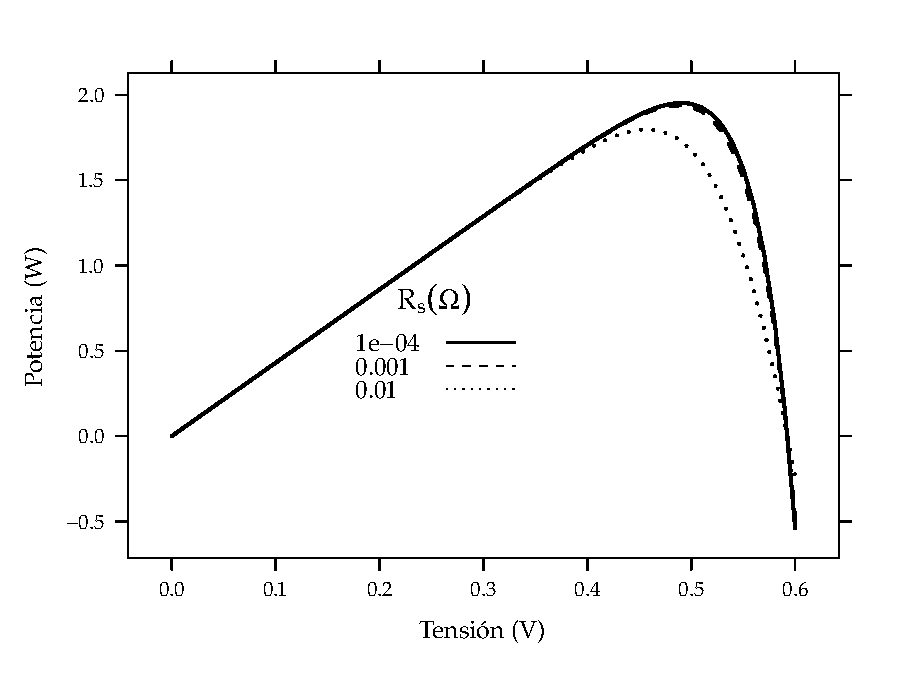
\includegraphics[width=.9\linewidth]{../figs/InfluenciaRs_Potencia.pdf}
\end{center}
\end{frame}

\begin{frame}[label={sec:orge611b91}]{Resistencia paralelo: Curva IV}
\begin{itemize}
\item Fugas de corriente en bordes de célula

\item Cortocircuitos metálicos

\item Caminos de difusión en fronteras de grano
\end{itemize}

\begin{center}
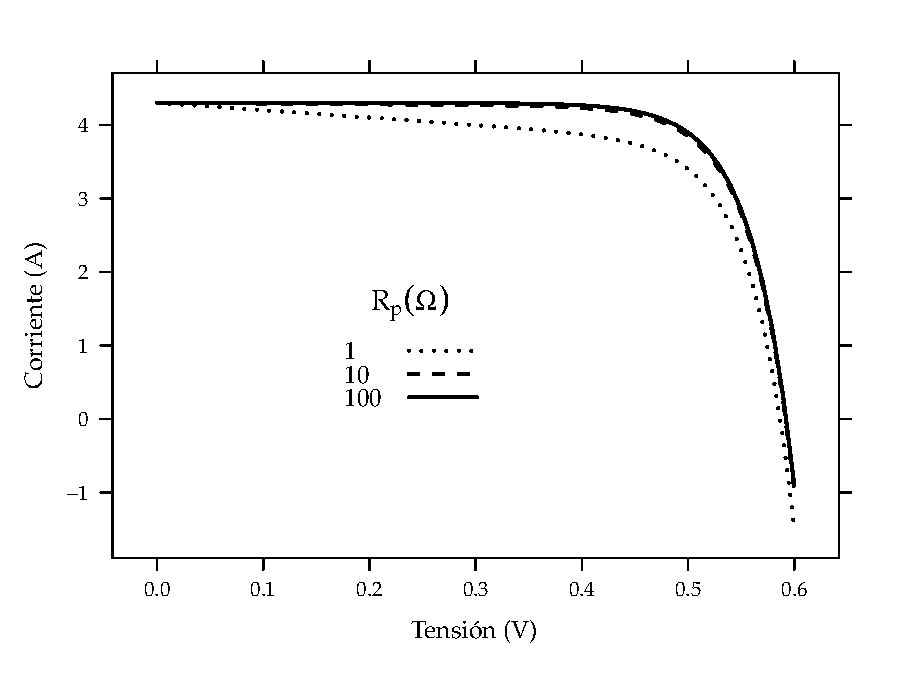
\includegraphics[width=.9\linewidth]{../figs/InfluenciaRsh_IV.pdf}
\end{center}
\end{frame}

\begin{frame}[label={sec:org0f28649}]{Resistencia paralelo: Curva PV}
\begin{itemize}
\item Fugas de corriente en bordes de célula

\item Cortocircuitos metálicos

\item Caminos de difusión en fronteras de grano
\end{itemize}

\begin{center}
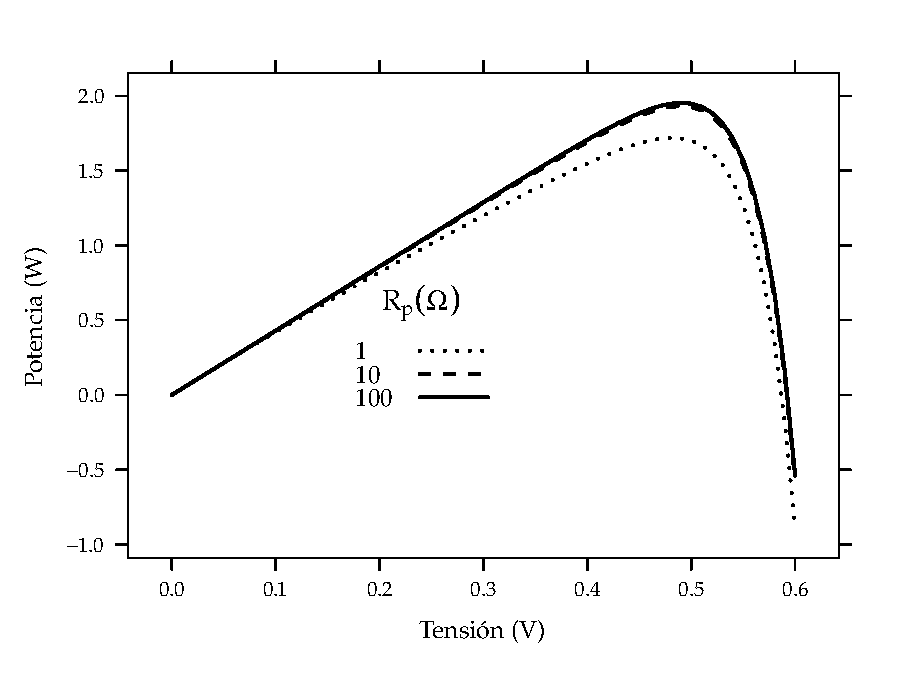
\includegraphics[width=.9\linewidth]{../figs/InfluenciaRsh_Potencia.pdf}
\end{center}
\end{frame}

\section{Fabricación}
\label{sec:org1322c01}

\begin{frame}[label={sec:orgc98c545}]{}
\begin{center}
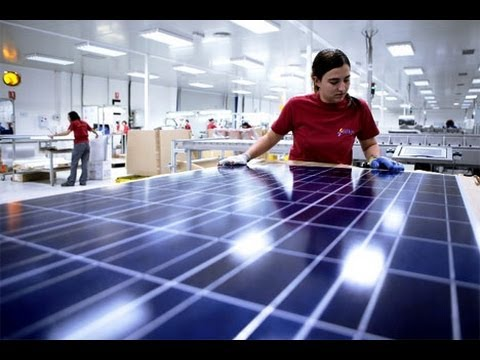
\includegraphics[width=.9\linewidth]{/home/oscar/github/esf/figs/solar_cell_manufacturing_video.jpg}
\end{center}

\begin{center}


\url{https://www.youtube.com/watch?v=BZKEkwOJ9Nw}

\url{https://www.youtube.com/watch?v=fZ1SC-vUe\_I}
\end{center}
\end{frame}

\begin{frame}[label={sec:org8dd2aa8}]{Purificación de silicio}
\begin{itemize}
\item El silicio puede extraerse de la cuarzita obteniendo Silicio de grado metalúrgico (98\% pureza).

\item Para la industria de la electrónica se necesita silicio de grado electronico (nivel de impureza por debajo de \(10^{-9}\), 9 nueves).

\item Para las células solares puede utilizarse silicio de grado solar (nivel de impureza algo mayor, \(10^{-5}\), 5 nueves).

\item Al mezclar silicio con acido clorhídrico se produce triclorosilano, que es destilado para eliminar impurezas.

\item Al unir silano de cloro con hidrógeno se obtiene de vuelta silicio, válido para células policristalinas (varios cristales en cada célula)
\end{itemize}
\end{frame}

\begin{frame}[label={sec:orgac4a595}]{Formación de obleas}
\begin{itemize}
\item Para obtener mayor pureza se emplea el silicio monocristalino (un sólo cristal) obtenido mediante el proceso de Czochralski o similar (se utiliza una semilla de cristal para crecer silicio a muy alta temperatura).

\item El lingote resultante debe ser cortado en obleas de \(200-500\,\mu m\).

\item Las obleas son sometidas a limpieza para eliminar impurezas por el cortado.

\item A continuación, son dopadas con Fósforo y Boro para crear la unión p-n.

\item Se limpian los bordes para evitar la formación de cortocircuitos entre las zonas p y n.
\end{itemize}
\end{frame}

\begin{frame}[label={sec:org3761be6}]{Formación de células}
\begin{itemize}
\item Se añaden los contactos posterior (alto recubrimiento) y anterior (optimización para obtener baja \(R_{s}\) y poco sombreado) empleando aleaciones de plata y aluminio.

\item Para reducir las pérdidas por reflexión se añade una capa antireflectante con (p.ej) óxido de Titanio (color azulado).

\item Si es posible, se textura la superficie (creación de mini pirámides).
\end{itemize}
\end{frame}
\end{document}